\documentclass[
11pt, % The default document font size, options: 10pt, 11pt, 12pt
%codirector, % Uncomment to add a codirector to the title page
]{charter} 




% El títulos de la memoria, se usa en la carátula y se puede usar el cualquier lugar del documento con el comando \ttitle
\titulo{Monitoreo y gestión remota de red de sensores Bluetooth en invernaderos} 

% Nombre del posgrado, se usa en la carátula y se puede usar el cualquier lugar del documento con el comando \degreename
%\posgrado{Carrera de Especialización en Sistemas Embebidos} 
\posgrado{Carrera de Especialización en Internet de las Cosas} 
%\posgrado{Carrera de Especialización en Intelegencia Artificial}
%\posgrado{Maestría en Sistemas Embebidos} 
%\posgrado{Maestría en Internet de las cosas}

% Tu nombre, se puede usar el cualquier lugar del documento con el comando \authorname
\autor{Ing. Facundo Andrioli Villa} 

% El nombre del director y co-director, se puede usar el cualquier lugar del documento con el comando \supname y \cosupname y \pertesupname y \pertecosupname
\director{Dr. Pablo Ventura}
\pertenenciaDirector{KeyLab} 
% FIXME:NO IMPLEMENTADO EL CODIRECTOR ni su pertenencia
\codirector{John Doe} % para que aparezca en la portada se debe descomentar la opción codirector en el documentclass
\pertenenciaCoDirector{FIUBA}

% Nombre del cliente, quien va a aprobar los resultados del proyecto, se puede usar con el comando \clientename y \empclientename
\cliente{Sr. Pablo Lodetti}
\empresaCliente{Wentux Tecnoagro}

% Nombre y pertenencia de los jurados, se pueden usar el cualquier lugar del documento con el comando \jurunoname, \jurdosname y \jurtresname y \perteunoname, \pertedosname y \pertetresname.
\juradoUno{Nombre y Apellido (1)}
\pertenenciaJurUno{pertenencia (1)} 
\juradoDos{Nombre y Apellido (2)}
\pertenenciaJurDos{pertenencia (2)}
\juradoTres{Nombre y Apellido (3)}
\pertenenciaJurTres{pertenencia (3)}
 
\fechaINICIO{17 de octubre de 2023}		%Fecha de inicio de la cursada de GdP \fechaInicioName
\fechaFINALPlan{5 de diciembre 2023} 	%Fecha de final de cursada de GdP
\fechaFINALTrabajo{10 de octubre 2024}	%Fecha de defensa pública del trabajo final


\begin{document}

\maketitle
\thispagestyle{empty}
\pagebreak


\thispagestyle{empty}
{\setlength{\parskip}{0pt}
\tableofcontents{}
}
\pagebreak


\section*{Registros de cambios}
\label{sec:registro}


\begin{table}[ht]
\label{tab:registro}
\centering
\begin{tabularx}{\linewidth}{@{}|c|X|c|@{}}
\hline
\rowcolor[HTML]{C0C0C0} 
Revisión & \multicolumn{1}{c|}{\cellcolor[HTML]{C0C0C0}Detalles de los cambios realizados} & Fecha      \\ \hline
0      & Creación del documento                                 &\fechaInicioName \\ \hline
1      & Se completa hasta el punto 5 inclusive                 & 31 de octubre de 2023 \\ \hline
2      & Se completa hasta el punto 9 inclusive                 & 07 de noviembre de 2023 \\ \hline
3	   & Se completa hasta el punto 12 inclusive                & 14 de noviembre de 2023 \\ \hline
4	   & Se completa hasta el punto 15 inclusive                & 21 de noviembre de 2023 \\ \hline
4.1	   & Finalización del documento                			   & 28 de noviembre de 2023 \\ \hline
%		  En distintas líneas \newline
%		  Así                                                    & dd/mm/aaaa \\ \hline
%3      & Se completa hasta el punto 11 inclusive                & dd/mm/aaaa \\ \hline
%4      & Se completa el plan	                                 & dd/mm/aaaa \\ \hline
\end{tabularx}
\end{table}

\pagebreak



\section*{Acta de constitución del proyecto}
\label{sec:acta}

\begin{flushright}
Buenos Aires, \fechaInicioName
\end{flushright}

\vspace{2cm}

Por medio de la presente se acuerda con el Ing. \authorname\hspace{1px} que su Trabajo Final de la \degreename\hspace{1px} se titulará ``\ttitle'', consistirá esencialmente en la implementación de una red de sensores Bluetooth, el desarrollo de una aplicación web progresiva y la configuración de un servidor IoT, y tendrá un presupuesto preliminar estimado de 640 h de trabajo y \$10201100 de pesos, con fecha de inicio \fechaInicioName\hspace{1px} y fecha de presentación pública \fechaFinalName.

Se adjunta a esta acta la planificación inicial.

\vfill

% Esta parte se construye sola con la información que hayan cargado en el preámbulo del documento y no debe modificarla
\begin{table}[ht]
\centering
\begin{tabular}{ccc}
\begin{tabular}[c]{@{}c@{}}Dr. Ing. Ariel Lutenberg \\ Director posgrado FIUBA\end{tabular} & \hspace{2cm} & \begin{tabular}[c]{@{}c@{}}\clientename \\ \empclientename \end{tabular} \vspace{2.5cm} \\ 
\multicolumn{3}{c}{\begin{tabular}[c]{@{}c@{}} \supname \\ Director del Trabajo Final\end{tabular}} \vspace{2.5cm} \\
%\begin{tabular}[c]{@{}c@{}}\jurunoname \\ Jurado del Trabajo Final\end{tabular}     &  & \begin{tabular}[c]{@{}c@{}}\jurdosname\\ Jurado del Trabajo Final\end{tabular}  \vspace{2.5cm}  \\
%\multicolumn{3}{c}{\begin{tabular}[c]{@{}c@{}} \jurtresname\\ Jurado del Trabajo Final\end{tabular}} \vspace{.5cm}                                                                     
\end{tabular}
\end{table}




\section{1. Descripción técnica-conceptual del proyecto a realizar}
\label{sec:descripcion}

La producción agrícola en invernaderos ha experimentado una transformación significativa a lo largo del tiempo. La necesidad de un control más preciso y eficiente del entorno de cultivo se ha vuelto esencial para asegurar la calidad y la productividad de las cosechas. La demanda de cultivos de alta calidad y el crecimiento de la población mundial han intensificado la presión sobre la industria agrícola para maximizar la producción. En este contexto, el monitoreo y la gestión de invernaderos se han convertido en cuestiones primordiales.

Sin embargo, enfrentar desafíos logísticos y técnicos, especialmente al supervisar y controlar múltiples invernaderos distribuidos en diversas ubicaciones, se ha convertido en un reto clave. La gestión descentralizada de invernaderos dispersos geográficamente ha presentado dificultades en la obtención de datos en tiempo real, la implementación de un control eficiente y la gestión unificada. La falta de soluciones integrales para abordar estos desafíos ha sido una limitación en la industria agrícola.

El proyecto se realiza en colaboración con la empresa argentina "Wentux Tecnoagro", que se especializa en la fabricación y desarrollo de controladores para salas de cultivo y automatización de procesos para garantizar cosechas seguras.

La solución que se propone implica la implementación de una red de sensores Bluetooth en invernaderos, junto con el desarrollo de una aplicación web progresiva (PWA) para el monitoreo local y un servidor IoT para la gestión remota de datos. Estos sensores recopilarán información sobre el clima y otros parámetros en tiempo real. La PWA permitirá a los usuarios acceder a estos datos y controlar los invernaderos desde cualquier lugar, mientras que el servidor IoT facilitará la gestión de datos y alarmas.

La propuesta de valor radica en satisfacer las necesidades de Wentux Tecnoagro y sus clientes, quienes primordialmente buscan tener un control total sobre sus cosechas y mantener un entorno de cultivo seguro. El proyecto se distingue por su capacidad de monitoreo y control remoto, permitiendo a los agricultores y profesionales de la agricultura gestionar sus invernaderos de manera eficiente y precisa.

La importancia del trabajo radica en la capacidad de impulsar la industria agrícola al proporcionar una solución avanzada para el monitoreo y la gestión de invernaderos, mejorando la calidad y la productividad de las cosechas, lo que es esencial para la seguridad alimentaria en un mundo en crecimiento.

En la figura 1, que se presenta a continuación, se muestra el diagrama en bloques del sistema, en el que se pueden observar:

\begin{itemize}
	\item Red de Sensores Bluetooth: recopila datos del entorno del invernadero.
	\item Módulo Central: recibe datos de los sensores Bluetooth y los envía al servidor a través de MQTT.
	\item Comunicación MQTT: facilita la transferencia de datos entre el módulo central y el servidor.
	\item Servidor IoT: almacena y procesa los datos recibidos de los sensores.
	\item PWA: permite el monitoreo y control del sistema en la red local.
	\item Nodos sensores y actuadores: recopilan datos y controlan dispositivos en el invernadero.
	\item Usuario remoto: accede a los datos recopilados a través del servidor IoT.
\end{itemize}


\begin{figure}[htpb]
\centering 
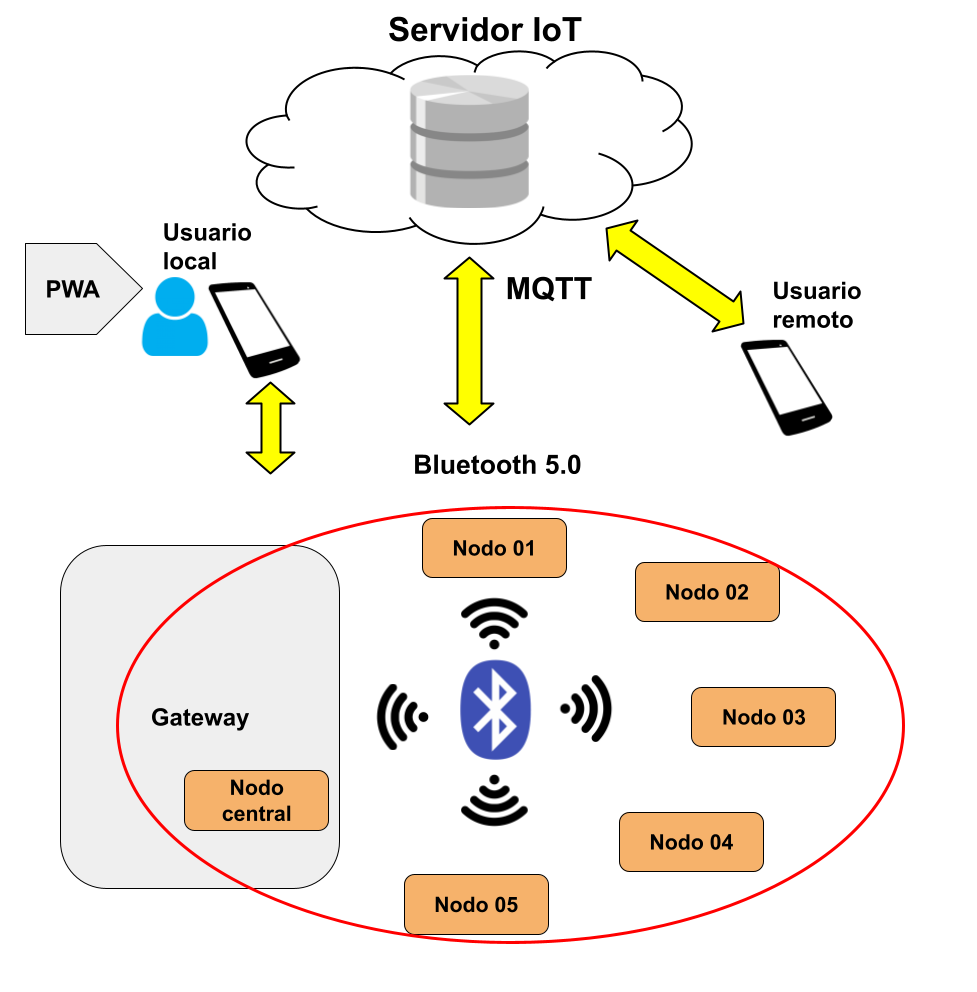
\includegraphics[width=.6\textwidth]{./Figuras/DiagramaNuevo.png}
\caption{Diagrama en bloques del sistema.}
\label{fig:diagBloques}
\end{figure}

\vspace{25px}



\section{2. Identificación y análisis de los interesados}
\label{sec:interesados}

\begin{table}[ht]
%\caption{Identificación de los interesados}
%\label{tab:interesados}
\begin{tabularx}{\linewidth}{@{}|l|X|X|l|@{}}
\hline
\rowcolor[HTML]{C0C0C0} 
Rol           & Nombre y Apellido & Organización 	& Puesto 	\\ \hline
Cliente       & \clientename      &\empclientename	&   -     	\\ \hline
Responsable   & \authorname       & FIUBA        	& Alumno 	\\ \hline
Orientador    & \supname	      & \pertesupname 	& Director Trabajo final \\ \hline
Usuario final &  Agricultores     &         -     	&    -    	\\ \hline
\end{tabularx}
\end{table}

\begin{itemize}
	\item Orientador: el Dr. Pablo Ventura, con su extensa experiencia, colaborará en la revisión y planificación del proyecto.
	\item Usuario final: agricultores que requieran gestionar sus invernaderos de manera eficiente y
precisa. 
\end{itemize}


\section{3. Propósito del proyecto}
\label{sec:proposito}

El propósito del proyecto consiste en la implementación de una red de sensores Bluetooth en invernaderos para recopilar información en tiempo real. Además, se desarrollará una PWA para el monitoreo local y se establecerá un servidor IoT en la nube para la gestión remota de datos.


\section{4. Alcance del proyecto}
\label{sec:alcance}

Dentro del alcance de este proyecto se incluye:

\begin{itemize}
	\item Diseño y desarrollo de un protocolo de comunicación basado en Bluetooth 5.0 entre los nodos sensores y el sistema embebido central.
	\item Creación de una PWA para el monitoreo local de los equipos en los invernaderos.
	\item Implementación de un servidor en la nube para el almacenamiento y gestión de datos recopilados por los sensores.
	\item Establecimiento de la comunicación cliente-servidor a través del protocolo MQTT para la transmisión de datos desde el sistema embebido central al servidor en la nube.
	\item Posibilidad de control remoto de los invernaderos y sus dispositivos desde la aplicación web.
	\item Gestión de alarmas y administración de los datos recibidos por los dispositivos conectados.
\end{itemize}

El presente proyecto no incluye:

\begin{itemize}
	\item El desarrollo del hardware del sistema embebido central, que ya está funcionando.
	\item Mantenimiento y actualizaciones a largo plazo del sistema.
\end{itemize}



\section{5. Supuestos del proyecto}
\label{sec:supuestos}


Para el desarrollo del presente proyecto se supone que: 

\begin{itemize}
	\item Se dispondrá del conocimiento necesario para desarrollar PWA y configurar el servidor en la nube.
	\item No habrá dificultades para conseguir el módulo ESP32 de Espressif Systems.
	\item Se dispondrá de acceso a la tecnología Bluetooth 5.0 para la comunicación entre los nodos sensores y el sistema embebido central.
	\item  Se tendrá acceso a una conexión a Internet estable para permitir la comunicación remota entre el sistema embebido central y el servidor en la nube mediante el protocolo MQTT.
	\item Se contará con la colaboración del cliente para la evaluación de las pruebas.
	\item Se contará con el tiempo suficiente para realizar las distintas tareas.
	\item La organización Wentux estará dispuesta a proporcionar el apoyo necesario y la colaboración requerida para el éxito del proyecto.
\end{itemize}




\section{6. Requerimientos}
\label{sec:requerimientos}



\begin{enumerate}
	\item Requerimientos funcionales
		\begin{enumerate}
			\item El sistema debe permitir que los módulos Bluetooth Low Energy (BLE) se comuniquen con el módulo central y puedan intercambiar datos.
			\item Los módulos BLE deben contar con una configuración de bajo consumo para permitir su uso con baterías.
			\item El usuario deberá tener la capacidad de habilitar o deshabilitar los distintos módulos disponibles.
			\item El módulo central debe ser capaz de auto detectar los módulos que estén dentro de su alcance.
			\item Se implementará un servidor en la nube con el software OpenRemote para el monitoreo remoto de los datos.
			\item El módulo central se conectará al servidor en la nube a través del protocolo MQTT.
		\end{enumerate}
	\item Requerimientos de documentación
		\begin{enumerate}
			\item Se documentarán las bibliotecas para implementar la red de sensores. 
			\item Se documentará el proceso general del desarrollo de la PWA y sus bibliotecas y/o frameworks utilizados.
			\item Se documentará el procedimiento de instalación y puesta en marcha del software OpenRemote y sus dependencias en el servidor remoto.
		\end{enumerate}
	\item Requerimientos de la interfaz
		\begin{enumerate}
			\item La PWA será la interfaz principal para obtener los datos que se recolectan.
			\item La PWA configurará y monitoreará la red. 
			\item La PWA requerirá acceso con usuario y contraseña.
			\item  La PWA se comunicará mediante MQTT con el servidor IoT para permitir al usuario obtener datos desde ubicaciones remotas.
			\item La PWA deberá enviar comandos a través de MQTT al servidor  para ejecutar funciones solicitadas por el usuario.
		\end{enumerate}
	\item Requerimientos confidencialidad
		\begin{enumerate}
			\item Se deberá mantener confidencialidad sobre algunos aspectos de los secretos comerciales, métodos de trabajo y de la información.
			\item Se deberá comprometer a mantener en el futuro dicha conducta.
		\end{enumerate}
\end{enumerate}


\section{7. Historias de usuarios (\textit{Product backlog})}
\label{sec:backlog}


Se utilizó la asignación de \textit{story points} para evaluar las historias de usuario. El valor se determinó considerando los siguientes factores: complejidad, dificultad e incertidumbre asociada con la tarea. La escala aplicada a cada uno de estos es la siguiente:

\begin{itemize}
    \item Complejidad:
    \begin{itemize}
        \item Alta: 8
        \item Media: 3
        \item Baja: 1
    \end{itemize}
    \item Dificultad:
    \begin{itemize}
        \item Alta: 8
        \item Media: 3
        \item Baja: 1
    \end{itemize}
    \item Incertidumbre:
    \begin{itemize}
        \item Alta: 5
        \item Media: 3
        \item Baja: 1
    \end{itemize}
\end{itemize}


Para calcular los \textit{story points} sumaremos la puntuación otorgada a cada factor y luego redondearemos el resultado al número de la serie de Fibonacci más cercano.


\begin{itemize}
	\item Como usuario, quiero acceder a la PWA con mi usuario y contraseña. Complejidad: 3 - Dificultad: 3 - Incertidumbre: 1 - \textbf{\textit{Story points}}: 8
	\item Como usuario, quiero modificar mi configuración. Complejidad: 3 - Dificultad: 3 - Incertidumbre: 1 - \textbf{\textit{Story points}}: 8
	\item Como usuario, quiero poder ver un listado de mis invernaderos. Complejidad: 1 - Dificultad: 3 - Incertidumbre: 1 - \textbf{\textit{Story points}}: 5
	\item Como usuario, quiero poder agregar nuevas invernaderos. Complejidad: 1 - Dificultad: 3 - Incertidumbre: 1 - \textbf{\textit{Story points}}: 5
	\item Como usuario, quiero poder ver un listado de mis alarmas. Complejidad: 1 - Dificultad: 3 - Incertidumbre: 1 - \textbf{\textit{Story points}}: 5
	\item Como usuario, quiero poder agregar nuevas alarmas. Complejidad: 3 - Dificultad: 3 - Incertidumbre: 1 - \textbf{\textit{Story points}}: 8
	\item Como usuario, quiero poder eliminar mis alarmas. Complejidad: 1 - Dificultad: 3 - Incertidumbre: 1 - \textbf{\textit{Story points}}: 5
	\item Como usuario, quiero recibir una notificación cuando una alarma es disparada. Complejidad: 3 - Dificultad: 8 - Incertidumbre: 1 - \textbf{\textit{Story points}}: 13
	\item Como usuario, quiero poder acceder al histórico de alarmas disparadas. Complejidad: 1 - Dificultad: 3 - Incertidumbre: 1 - \textbf{\textit{Story points}}: 5
	\item Como encargado del proyecto, quiero que todas las comunicaciones de transferencia de datos empleen certificados TLS para asegurar la seguridad de los mismos. Complejidad: 8 - Dificultad: 8 - Incertidumbre: 3 - \textbf{\textit{Story points}}: 21
	\item Como encargado del proyecto, necesito que cualquier información confidencial se guarde de manera encriptada, con el fin de resguardar los datos contra accesos no autorizados. Complejidad: 3 - Dificultad: 3 - Incertidumbre: 3 - \textbf{\textit{Story points}}: 13.
\end{itemize}

\section{8. Entregables principales del proyecto}
\label{sec:entregables}


Los entregables del proyecto son:

\begin{itemize}
	\item Implementación de red de sensores Bluetooth.
	\item Implementación de la API REST.
	\item Desarrollo de una PWA.
	\item Configuración del sistema de comunicación MQTT.
	\item Implementación y despliegue del servidor de IoT.
	\item Elaboración de un manual de usuario.
	\item Informes de avances.
	\item Prototipo funcional.
	\item Informe final.
	\item Presentación del proyecto.
\end{itemize}



\section{9. Desglose del trabajo en tareas}
\label{sec:wbs}

\begin{enumerate}
\item Implementación de red de sensores Bluetooth (120 h).
	\begin{enumerate}
	\item Investigación del framework a utilizar (10 h).
	\item Investigación de la tecnología BLE (10 h).
	\item Diseño e implementación de la comunicación BLE (25 h).
	\item Comunicación con el módulo central (25 h).
	\item Implementación de sensores analógicos y digitales (20 h).
	\item Pruebas unitarias (10 h).
	\item Pruebas de integración (10 h).
	\item Documentación (10 h).
	\end{enumerate}
\item Desarrollo de la API REST (120 h).
	\begin{enumerate}
	\item Investigación de APIs (10 h).
	\item Implementación de la base de datos (25 h).
	\item Configuración de los protocolos (10 h).
	\item Definición y diseño de endpoints (20 h).
	\item Implementación de la API (35 h).
	\item Pruebas de integración (10 h).
	\item Documentación (10 h).
	\end{enumerate}
\item Desarrollo de una PWA (100 h).
	\begin{enumerate}
	\item Investigación de frameworks y bibliotecas a utilizar (15 h).
	\item Integración de la API diseñada (30 h).
	\item Diseño del frontend (35 h).
	\item Pruebas de integración (10 h).
	\item Documentación (10 h).
	\end{enumerate}
\item Configuración del sistema de comunicación MQTT (115 h).
	\begin{enumerate}
	\item Investigación del protocolo (10 h).
	\item Implementación y configuración de los certificados TLS (15 h).
	\item Configuración del broker (15 h).
	\item Configuración de los protocolos (15 h).
	\item Diseño y estructura de tópicos (30 h).
	\item Configuración de seguridad (20 h).
	\item Pruebas de integración (10 h).
	\end{enumerate}
\item Implementación y despliegue del servidor de IoT (130 h).
	\begin{enumerate}
	\item Investigación de la OpenRemote (15 h).
	\item Creación de un servidor en Google Cloud (15 h).
	\item Instalación de OpenRemote en el servidor (15 h).
	\item Configuración de OpenRemote (30 h).
	\item Conexión a MQTT (15 h).
	\item Generación de paneles de información (20 h).
	\item Pruebas de integración (10 h).
	\item Documentación (10 h).
	\end{enumerate}
\item Presentación del proyecto (55 h)
	\begin{enumerate}
	\item Escritura de la memoria del proyecto (40 h).
	\item Elaboración de la presentación (15 h).
	\end{enumerate}
\end{enumerate}

Cantidad total de horas: (640 h)


\section{10. Diagrama de Activity On Node}
\label{sec:AoN}

En el diagrama se puede observar en rojo el camino crítico y la unidad de tiempo está expresada en horas.

\begin{figure}[htpb]
\centering 
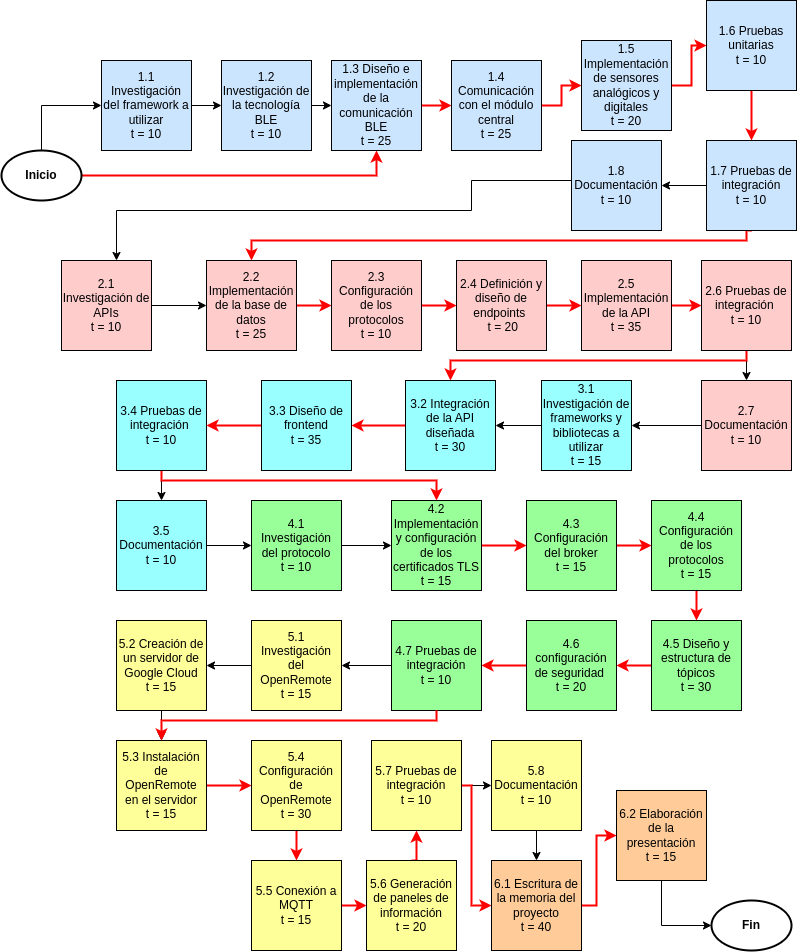
\includegraphics[width=1\textwidth]{./Figuras/diagrama_aon.png}
\caption{Diagrama de \textit{Activity on Node}.}
\label{fig:AoN}
\end{figure}

\begin{figure}[htpb]
\centering 
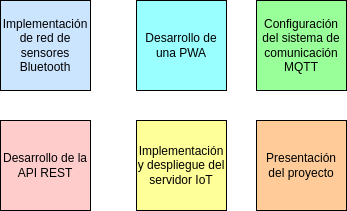
\includegraphics[width=0.4\textwidth]{./Figuras/referencias_aon.png}
\caption{Referencias del diagrama de \textit{Activity on Node}.}
\label{fig:AoN}
\end{figure}



\section{11. Diagrama de Gantt}
\label{sec:gantt}

\begin{figure}[htpb]
\centering 
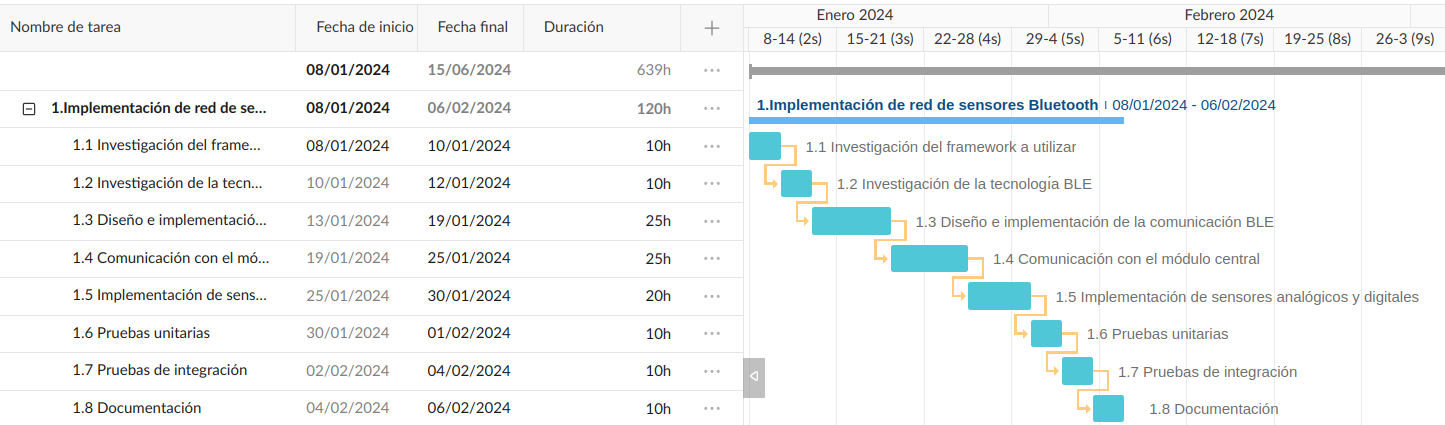
\includegraphics[width=1.1\textwidth]{./Figuras/diagrama_gantt_1.png}
\caption{Diagrama de Gantt parte 1 de 6.}
\label{fig:diagGrantt1}
\end{figure}
\vspace{5px}

\begin{figure}[htpb]
\centering 
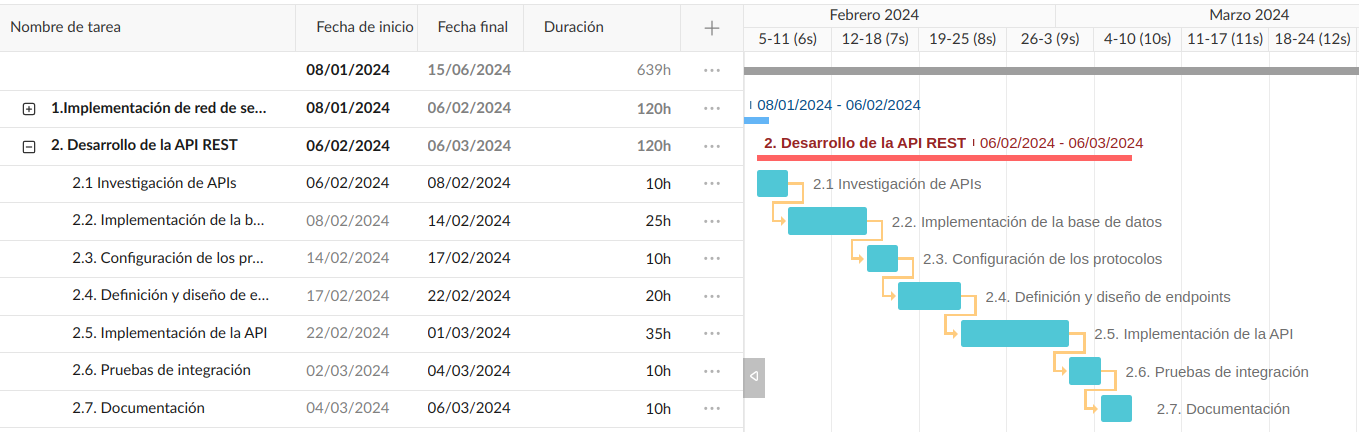
\includegraphics[width=1.1\textwidth]{./Figuras/diagrama_gantt_2.png}
\caption{Diagrama de Gantt parte 2 de 6.}
\label{fig:diagGrantt2}
\end{figure}
\vspace{5px}

\begin{figure}[htpb]
\centering 
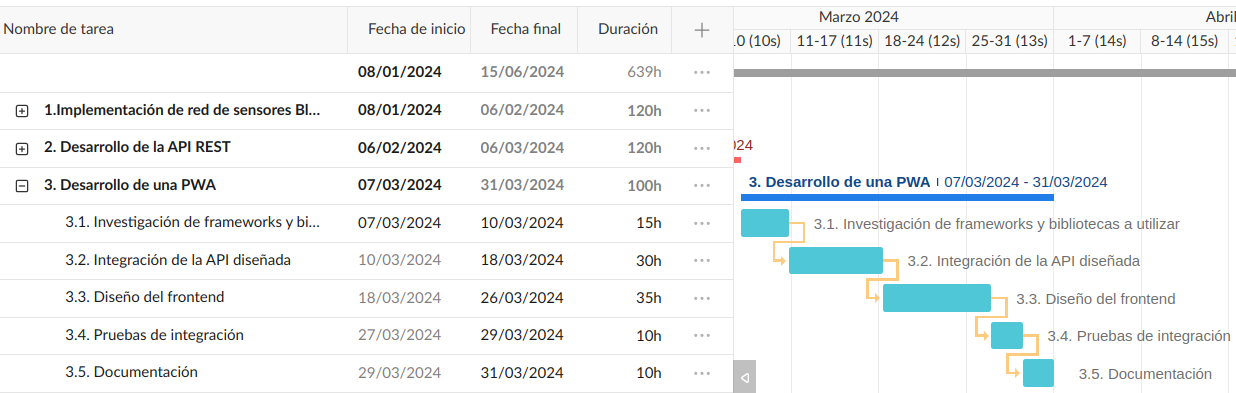
\includegraphics[width=1.1\textwidth]{./Figuras/diagrama_gantt_3.png}
\caption{Diagrama de Gantt parte 3 de 6.}
\label{fig:diagGrantt3}
\end{figure}
\vspace{5px}

\begin{figure}[htpb]
\centering 
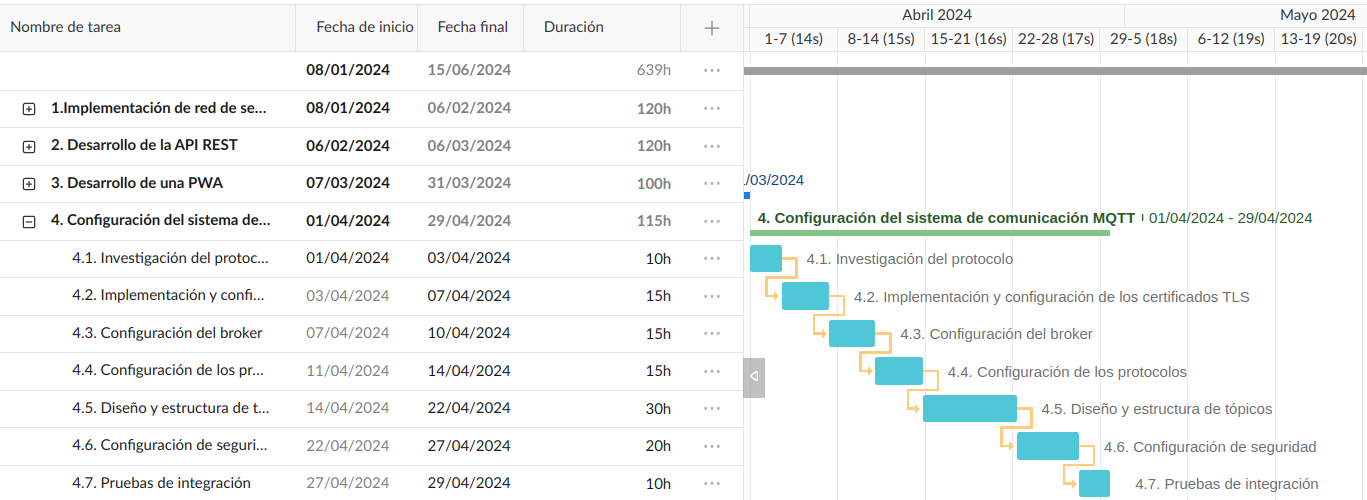
\includegraphics[width=1.1\textwidth]{./Figuras/diagrama_gantt_4.png}
\caption{Diagrama de Gantt parte 4 de 6.}
\label{fig:diagGrantt4}
\end{figure}
\vspace{5px}

\begin{figure}[htpb]
\centering 
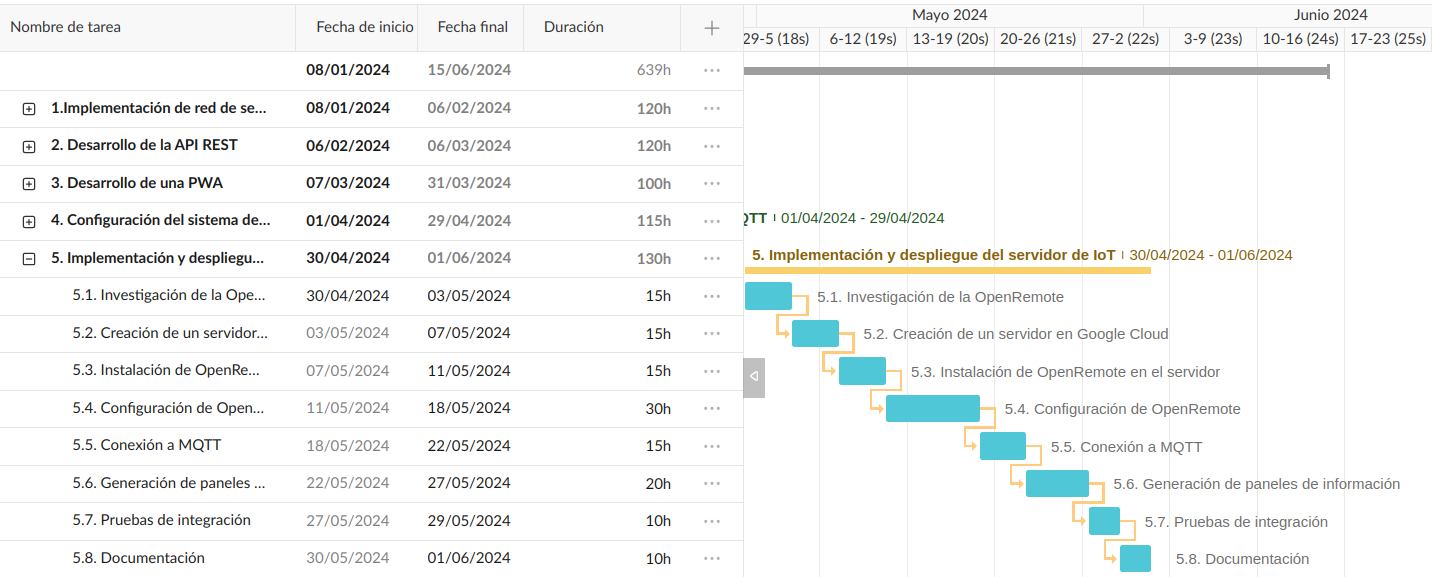
\includegraphics[width=1.1\textwidth]{./Figuras/diagrama_gantt_5.png}
\caption{Diagrama de Gantt parte 5 de 6.}
\label{fig:diagGrantt5}
\end{figure}
\vspace{5px}

\begin{figure}[htpb]
\centering 
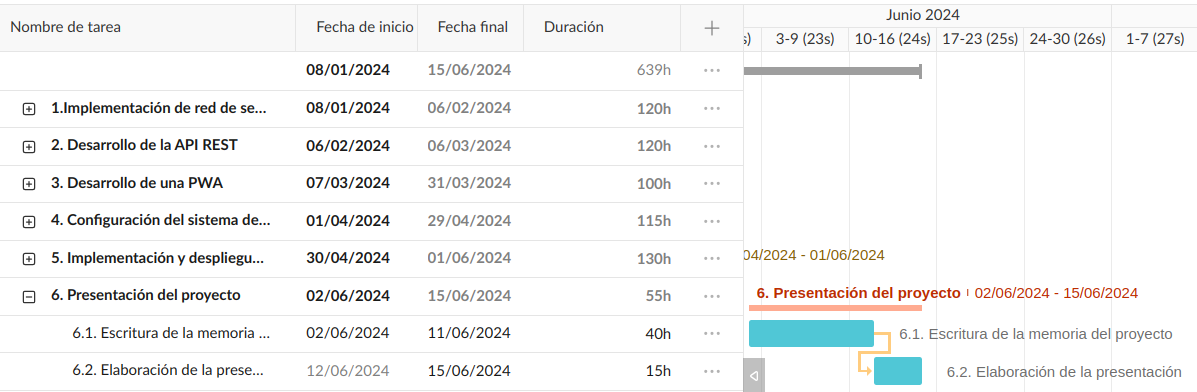
\includegraphics[width=1.1\textwidth]{./Figuras/diagrama_gantt_6.png}
\caption{Diagrama de Gantt parte 6 de 6.}
\label{fig:diagGrantt6}
\end{figure}
\vspace{5px}

\section{12. Presupuesto detallado del proyecto}
\label{sec:presupuesto}

El presupuesto del proyecto está estimado en pesos argentinos.

\begin{table}[htpb]
\centering
\begin{tabularx}{\linewidth}{@{}|X|c|r|r|@{}}
\hline
\rowcolor[HTML]{C0C0C0} 
\multicolumn{4}{|c|}{\cellcolor[HTML]{C0C0C0}COSTOS DIRECTOS} \\ \hline
\rowcolor[HTML]{C0C0C0} 
Descripción & 
  \multicolumn{1}{c|}{\cellcolor[HTML]{C0C0C0}Cantidad} &
  \multicolumn{1}{c|}{\cellcolor[HTML]{C0C0C0}Valor unitario} &
  \multicolumn{1}{c|}{\cellcolor[HTML]{C0C0C0}Valor total} \\ \hline
Horas de ingeniería & 
  \multicolumn{1}{c|}{640} &
  \multicolumn{1}{c|}{\$10000} &
  \multicolumn{1}{c|}{\$6400000} \\ \hline
Gateway &
  \multicolumn{1}{c|}{1} &
  \multicolumn{1}{c|}{\$400000} &
  \multicolumn{1}{c|}{\$400000} \\ \hline
Módulos BLE & 
  \multicolumn{1}{c|}{4} &
  \multicolumn{1}{c|}{\$150000} &
  \multicolumn{1}{c|}{\$600000} \\ \hline
Fuente múltiple 5 V USB & 
  \multicolumn{1}{c|}{1} &
  \multicolumn{1}{c|}{\$27000} &
  \multicolumn{1}{c|}{\$27000} \\ \hline
Fuente 5 V USB &
  \multicolumn{1}{c|}{4} &
  \multicolumn{1}{c|}{\$15000} &
  \multicolumn{1}{c|}{\$60000} \\ \hline
Servidor nube (mensual) &
  \multicolumn{1}{c|}{12} &
  \multicolumn{1}{c|}{\$30000} &
  \multicolumn{1}{c|}{\$360000} \\ \hline
\multicolumn{3}{|c|}{SUBTOTAL} &
  \multicolumn{1}{c|}{\$7847000} \\ \hline
\rowcolor[HTML]{C0C0C0} 
\multicolumn{4}{|c|}{\cellcolor[HTML]{C0C0C0}COSTOS INDIRECTOS} \\ \hline
\rowcolor[HTML]{C0C0C0} 
Descripción &
  \multicolumn{1}{c|}{\cellcolor[HTML]{C0C0C0}Cantidad} &
  \multicolumn{1}{c|}{\cellcolor[HTML]{C0C0C0}Valor unitario} &
  \multicolumn{1}{c|}{\cellcolor[HTML]{C0C0C0}Valor total} \\ \hline
30 \% de los costos directos  & 
  \multicolumn{1}{c|}{-} &
  \multicolumn{1}{c|}{-} &
  \multicolumn{1}{c|}{\$2354100} \\ \hline
\multicolumn{3}{|c|}{SUBTOTAL} &
  \multicolumn{1}{c|}{\$2354100} \\ \hline
\rowcolor[HTML]{C0C0C0}
\multicolumn{3}{|c|}{TOTAL} & \$10201100
   \\ \hline
\end{tabularx}%
\end{table}


\section{13. Gestión de riesgos}
\label{sec:riesgos}

\textbf{Identificación de los riesgos y estimación de sus consecuencias:}

Se analizan los riesgos del proyecto asignándoles valores del 1 al 10 en términos de su gravedad y probabilidad de ocurrencia. Se identificarán cinco posibles riesgos y se los evaluará en base a estos dos criterios.

Riesgo 1: insuficiente tiempo para finalizar el proyecto.
\begin{itemize}
	\item Severidad (S): 9. Si el tiempo no es suficiente, el proyecto se vería afectado y podría extenderse más allá del plazo previsto.
	\item Ocurrencia (O): 3. Se asignó una cantidad considerable de horas para poder finalizarlo en tiempo y forma.
\end{itemize}

Riesgo 2: posible pérdida del código del sistema.
\begin{itemize}
	\item Severidad (S): 9. Llevaría a la necesidad de volver a codificar.
	\item Ocurrencia (O): 2. Se implementará control de versiones con Git y se contará con un repositorio web.
\end{itemize}

Riesgo 3: selección incorrecta del microcontrolador.
\begin{itemize}
	\item Severidad (S): 6. Podría existir una limitación en la capacidad de recursos del componente elegido.
	\item Ocurrencia (O): 2. Se realizará una verificación exhaustiva para asegurarse de que el producto seleccionado satisfaga todas las necesidades identificadas en el proyecto.
\end{itemize}

Riesgo 4: surgimiento de una alternativa de biblioteca o framework superior al planificado.
\begin{itemize}
	\item Severidad (S): 1. Una nueva alternativa podría poner al producto en desventaja, aunque usar tecnologías probadas garantiza estabilidad.
	\item Ocurrencia (O): 9. En el campo de la informática, surgen constantemente nuevas opciones, aumentando la probabilidad de encontrar una solución superior a la planificada inicialmente.
\end{itemize}

Riesgo 5: fallas en los componentes electrónicos.
\begin{itemize}
	\item Severidad (S): 8. Si algún componente electrónico se encontrara defectuoso, se podrían producir retrasos en el proyecto y gastos adicionales.
	\item Ocurrencia (O): 3. Aunque es poco probable, siempre existe la posibilidad de recibir un componente defectuoso.
\end{itemize}


\textbf{Tabla de gestión de riesgos:      (El RPN se calcula como RPN=SxO)}

\begin{table}[htpb]
\centering
\begin{tabularx}{\linewidth}{@{}|X|c|c|c|c|c|c|@{}}
\hline
\rowcolor[HTML]{C0C0C0} 
Riesgo & S & O & RPN & S* & O* & RPN* \\ \hline
1. Insuficiente tiempo para finalizar el proyecto       & 9  & 3  &  27   &  8  & 2   &   16   \\ \hline
2. Posible pérdida del código del sistema.      & 9  & 1  &  9   &    &    &      \\ \hline
3. Selección incorrecta del microcontrolador.       & 6  & 2  &  12   &    &    &      \\ \hline
4. Surgimiento de una alternativa de biblioteca o framework superior al planificado.       & 1  & 9  &  9   &    &    &      \\ \hline
5. Fallas en los componentes electrónicos.       & 8  & 3  &  24   &  8  & 1   &  8    \\ \hline
\end{tabularx}%
\end{table}


Criterio adoptado: se tomarán medidas de mitigación en los riesgos cuyos números de RPN sean mayores a 20

Nota: los valores marcados con (*) en la tabla corresponden luego de haber aplicado la mitigación.


\textbf{Plan de mitigación de los riesgos que originalmente excedían el RPN máximo establecido:}

Riesgo 1: insuficiente tiempo para finalizar el proyecto.
\begin{itemize}
	\item Plan de mitigación: investigar en profundidad tecnologías desconocidas para anticipar posibles problemas y, de ser necesario, buscar ayuda de un experto.
	\item Severidad (S*): 8. Con el conocimiento de estas tecnologías, las tareas serán más eficientes y requerirán menos tiempo.
	\item Ocurrencia (O*): 2. Al comprender mejor estas tecnologías y contar con la asistencia de un experto, se reducen significativamente los riesgos de retrasos por falta de tiempo.
\end{itemize}

Riesgo 5: fallas en los componentes electrónicos.
\begin{itemize}
	\item Plan de mitigación: realizar pruebas exhaustivas antes del uso y trabajar con proveedores confiables que ofrezcan garantías sólidas.	
	\item Severidad (S): 8. La severidad se mantiene, ya que cualquier fallo en un componente resultaría en retrasos y gastos adicionales.
	\item Ocurrencia (O*): 1. Al contar con una lista actualizada de varios proveedores confiables, se reduce significativamente la posibilidad de ocurrencia de problemas.
\end{itemize}


\section{14. Gestión de la calidad}
\label{sec:calidad}


\begin{enumerate}
	\item Requerimientos funcionales
		\begin{enumerate}
			\item El sistema debe permitir que los módulos Bluetooth Low Energy (BLE) se comuniquen con el módulo central y puedan intercambiar datos.
			\begin{itemize}
				\item Verificación: tests automáticos para verificar la conectividad y el intercambio de datos entre los módulos BLE y el módulo central.
				\item Validación: el cliente intentará comunicar datos entre los módulos BLE y el módulo central para confirmar que la interacción funciona.
			\end{itemize}
			\item Los módulos BLE deben contar con una configuración de bajo consumo para permitir su uso con baterías.
			\begin{itemize}
				\item Verificación:  pruebas de consumo energético que demuestren el funcionamiento adecuado de los módulos BLE en modo de bajo consumo.
				\item Validación: el cliente verificará la duración de la batería en los módulos BLE configurados en modo de bajo consumo para asegurar que cumplen con la eficiencia energética necesaria.
			\end{itemize}
			\item El usuario deberá tener la capacidad de habilitar o deshabilitar los distintos módulos disponibles.
			\begin{itemize}
				\item Verificación: pruebas de interfaz de usuario para verificar la capacidad de activar y desactivar los módulos.
				\item Validación: el cliente utilizará la interfaz para activar y desactivar los módulos, comprobando la funcionalidad.
			\end{itemize}
			\item El módulo central debe ser capaz de auto detectar los módulos que estén dentro de su alcance.
			\begin{itemize}
				\item Verificación: pruebas de detección automática para asegurar que el módulo central identifica correctamente los módulos disponibles.
				\item Validación: el cliente observará la detección automática de los módulos en alcance para confirmar que el sistema realiza esta acción correctamente.
			\end{itemize}
			\item Se implementará un servidor en la nube con el software OpenRemote para el monitoreo remoto de los datos.
			\begin{itemize}
				\item Verificación: configuración exitosa del servidor en la nube con OpenRemote y pruebas de transmisión de datos.
				\item Validación: el cliente accederá al servidor remoto y verificará personalmente el monitoreo de los datos para confirmar que la implementación cumple con los requerimientos.
			\end{itemize}
			\item El módulo central se conectará al servidor en la nube a través del protocolo MQTT.
			\begin{itemize}
				\item Verificación: pruebas de conexión que validen el envío y recepción de datos entre el módulo central y el servidor utilizando MQTT.
				\item Validación: el cliente confirmará la comunicación exitosa entre el módulo central y el servidor a través del protocolo MQTT al observar el intercambio de datos.
			\end{itemize}
		\end{enumerate}
	\item Requerimientos de documentación
		\begin{enumerate}
			\item Se documentarán las bibliotecas para implementar la red de sensores.
			\begin{itemize}
				\item Verificación: revisión de la documentación generada para asegurar que detalla exhaustivamente el uso de las bibliotecas en la implementación de la red de sensores.
				\item Validación: el cliente intentará implementar la red de sensores siguiendo la documentación proporcionada para asegurar la comprensión y utilidad de la misma.
			\end{itemize} 
			\item Se documentará el proceso general del desarrollo de la PWA y sus bibliotecas y/o frameworks utilizados.
			\begin{itemize}
				\item Verificación: revisión de la documentación para confirmar que abarca el proceso completo de desarrollo de la PWA, incluyendo bibliotecas y frameworks utilizados, y proporciona una guía detallada.
				\item Validación: el cliente revisará la documentación y tratará de seguir los pasos para comprender el proceso de desarrollo de la PWA, evaluando la claridad y amplitud de la documentación.
			\end{itemize}
			\item Se documentará el procedimiento de instalación y puesta en marcha del software OpenRemote y sus dependencias en el servidor remoto.
			\begin{itemize}
				\item Verificación: revisión de la documentación para asegurar que contiene pasos claros y detallados para la instalación del software OpenRemote y sus dependencias en el servidor remoto.
				\item Validación: el cliente intentará seguir la documentación proporcionada para instalar el software OpenRemote y sus dependencias en un servidor remoto, asegurándose de que la documentación sea comprensible y efectiva.
			\end{itemize}
		\end{enumerate}
	\item Requerimientos de la interfaz
		\begin{enumerate}
			\item La PWA será la interfaz principal para obtener los datos que se recolectan.
			\begin{itemize}
				\item Verificación: pruebas de acceso y visualización de datos a través de la PWA.
				\item Validación: el cliente accederá a la PWA para obtener y revisar los datos recolectados, confirmando que la PWA proporciona la información de manera clara y accesible.
			\end{itemize}
			\item La PWA configurará y monitoreará la red.
			\begin{itemize}
				\item Verificación: pruebas que demuestren la capacidad de configurar la red y monitorearla a través de la PWA.
				\item Validación: el cliente intentará configurar la red y monitorearla utilizando la PWA, verificando que pueda realizar estas acciones de manera efectiva y sin dificultades.
			\end{itemize} 
			\item La PWA requerirá acceso con usuario y contraseña.
			\begin{itemize}
				\item Verificación: pruebas de autenticación mediante usuario y contraseña en la PWA.
				\item Validación: el cliente intentará acceder a la PWA utilizando credenciales de usuario y contraseña, asegurándose de que el proceso de autenticación funcione correctamente.
			\end{itemize}
			\item  La PWA se comunicará mediante MQTT con el servidor IoT para permitir al usuario obtener datos desde ubicaciones remotas.
			\begin{itemize}
				\item Verificación: pruebas de comunicación exitosa entre la PWA y el servidor IoT a través de MQTT.
				\item Validación: el cliente intentará acceder a la PWA desde ubicaciones remotas y verificará que pueda obtener datos, confirmando que la comunicación a través de MQTT funciona según lo esperado.
			\end{itemize}
			\item La PWA deberá enviar comandos a través de MQTT al servidor  para ejecutar funciones solicitadas por el usuario.
			\begin{itemize}
				\item Verificación: pruebas que demuestren la capacidad de la PWA para enviar comandos al servidor mediante MQTT.
				\item Validación: el cliente intentará enviar comandos desde la PWA al servidor a través de MQTT, verificando que las funciones solicitadas se ejecuten correctamente.
			\end{itemize}
		\end{enumerate}
\end{enumerate}

\section{15. Procesos de cierre}    
\label{sec:cierre}

Las actividades asociadas al cierre estarán a cargo del responsable del proyecto, Facundo Andrioli Villa

\begin{itemize}
	\item Se analizará si los tiempos que realmente tomó realizar una tarea coinciden con los tiempos que se habían planeado previamente.
	\item Se comprobará si todos los requerimientos pedidos por el cliente fueron cumplidos por completo.
	\item Se analizarán las técnicas y procedimientos que fueron efectivos o no para lograr los objetivos del proyecto.
	\item Cada problema o contratiempo que haya causado un desvío en el curso normal del proyecto será identificado, junto con sus soluciones correspondientes.
	\item Se llevará a cabo una exposición formal del proyecto, durante la cual se expresará gratitud a todas las personas involucradas, incluyendo miembros del jurado, profesores y autoridades de la CEIoT.
\end{itemize}


\end{document}
